\documentclass[10pt,a4paper]{article} 
\fontfamily{cmss}
\usepackage{amsmath}
\usepackage{amssymb}
\usepackage{mathtools}
\usepackage[brazilian]{babel}
\usepackage[utf8]{inputenc}
\usepackage[T1]{fontenc}
\usepackage[parfill]{parskip}
\usepackage[margin=1.0in]{geometry}
\usepackage{graphicx}
\usepackage{type1ec}
\usepackage{graphicx}
\usepackage{listings}
\usepackage[Algoritmo]{algorithm}
\usepackage[noend]{algpseudocode}
\usepackage{booktabs}
\usepackage{multirow,tabularx}
\usepackage[table,xcdraw]{xcolor}

\usepackage{makecell}
\renewcommand\theadalign{tc}
\renewcommand\theadfont{\bfseries}
\renewcommand\theadgape{\Gape[4pt]}
\renewcommand\cellgape{\Gape[4pt]}

\begin{document}

	% CABECALHO %

	\begin{minipage}[b]{0.05\linewidth}
		
\includegraphics[scale=0.3]{ufmg}
	\end{minipage}
	\hfill
	\begin{minipage}[b]{0.95\linewidth}
		\begin{flushright}
			\textbf{UNIVERSIDADE FEDERAL DE MINAS GERAIS} \\
			\textsc{Graduação em Engenharia de Sistemas} \\
			\textbf{Algoritmos e Estruturas de Dados III - Trabalho Prático 2} \\
			Uaibucks \\
			Matheus Silva Araujo - 2013066265
		\end{flushright}
	\end{minipage}

	\begin{center}
		\hrulefill
	\end{center}

	% CABECALHO %

	\section{Introdução}

	No Trabalho Prático 2 da disciplina de Algoritmos e Estruturas de Dados III, nosso velho conhecido Nubby abriu uma startup de consultoria e 
	tem a famosa cafeteria \emph{Uaibucks} como cliente. Essa cafeteria deseja instalar-se em uma nova cidade, e para isso impôs algumas restrições. 

	A cidade possui $N$ esquinas, duas esquinas são vizinhas se há uma rua que as interligue. Cada esquina possui uma demanda associada $d_i \in \mathbb{N}$.
	A empresa deseja abrir cafeterias em um subconjunto de esquinas, tais que duas cafeterias não estejam em esquinas vizinhas e a demanda esperada seja máxima.

	Para este trabalho, é necessário:

	\begin{itemize}

		\item Modelar o problema utilizando teoria de grafos;
		\item Provar que o problema pode ser modelado como um problema de decisão;
		\item Provar que o problema de decisão é um problema NP-Complemento;
		\item Implementar um algoritmo exato que resolva o problema;
		\item Implementar uma heurística para o problema.

	\end{itemize}

	\section{Grafo}

	O problema da \emph{Uaibucks} pode ser modelado através de um grafo, $G = (V,A)$, não direcionado, ponderado nos vértices.

	Para a entrada de exemplo do enunciado, o grafo é apresentado na Figura \ref{fig_grafo01}.

	\begin{figure}[H]
		\centering
		\caption{Modelagem em Grafo}
		\label{fig_grafo01}
		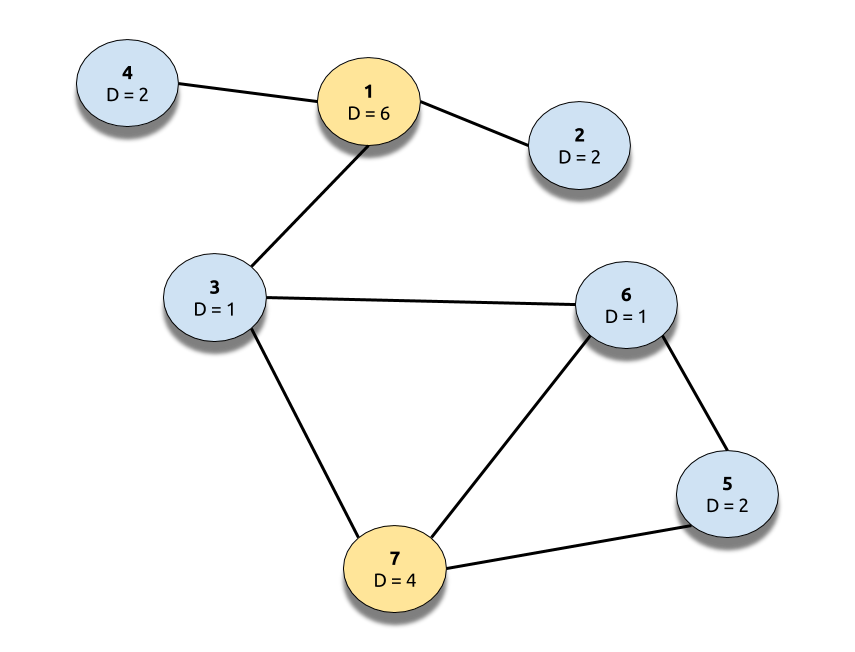
\includegraphics[scale=0.35]{grafo}
	\end{figure}

	Os critérios estabelecidos pela \emph{Uaibucks} definem o que é conhecido em Teoria dos Grafos como \emph{Conjunto Dominante}.

	Um conjunto dominante $D$ em um grafo é um conjunto tal que qualquer vértice $v$ do grafo ou está no conjunto $D$ ou é adjacente a pelo menos um 
	vértice contido no conjunto.

	\section{Problema de decisão}

	O problema apresentado é essencialmente um problema de otimização. 
	Deseja-se encontrar um \emph{Conjunto Dominante} que tenha demanda total máxima.

	No entanto, é possível transformá-lo em um problema de decisão do tipo: caso a demanda máxima encontrada seja maior que um valor $k$, 
	a empresa irá se instalar na cidade; caso contrário, não irá se instalar.

    \section{NP-Completude}

    O problema de encontrar um \emph{Conjunto Dominante}, $CD$, é um problema de decisão \emph{NP-Completo}.

    Para provar isso, o primeiro passo é mostrar um algoritmo determinista polinomial que verifica o conjunto dominante, Algoritmo \ref{alg01}.

    \begin{algorithm}[H]
    	\caption{Verifica $CD$}
    	\label{alg01}

    	\begin{algorithmic}[1]
    		
    		\If {|S| > n}
    			\State return FALSE
    		\EndIf

    		\For{i = 1 to |V|}
    			\If {V[i] $\notin$ S}
    				\State adj = FALSE
    				\For {$j$ in S}
    					\If {V[i], $j$ $\in$ A}
    						\State adj = TRUE
						\EndIf
					\EndFor
    				\If {adj = FALSE} 
    					\State return FALSE
					\EndIf
    			\EndIf
    		\EndFor

    		\State return TRUE

		\end{algorithmic}
        
    \end{algorithm}

    O próximo passo é mostrar que existe um problema $\pi \in $ \emph{NP-Completo} que possa ser transformado no \emph{Problema do Conjunto Dominante}.

    Para isso, será usado o problema da \emph{Cobertura de Vértices}, $CV$, conhecidamente \emph{NP-Completo}.

    Inicialmente, deve-se converter o grafo $G(V,A)$ com um valor $k$ do problema $CV$, em um grafo $G'(V',A')$ para o problema $CD$ com um valor $n$.

    Define-se $n$ e $k$.

    Para construir $G'$ em tempo polinomial:

    \begin{itemize}

    	\item Todo vértice de $G$ também é vértice de $G'$.
    	\item Toda aresta de $G$ também é aresta de $G'$.
    	\item Para cada aresta (i,j) $\in$ A, cria-se um vértice $z_{ij}$ em $G$ e adicionam-se duas novas arestas (i, $z_{ij}$) e ($z_{ij}$, j).

    \end{itemize}

    Se $G$ tem cobertura de vértice menor ou igual $k$, $G'$ tem conjunto dominante de tamanho menor ou igual a $n$.

    Se $G'$ tem $CD$ de tamanho menor ou igual a $n$, $G$ terá $CV$ de tamanho menor ou igual a $k$.

	\section{Algoritmo Exato}

	O Algoritmo Exato implementado para resolver o problema tem a seguinte estrutura: 

	\begin{itemize}
		\item Gerar todos os subconjuntos possíveis do grafo, complexidade $O(2^n)$, onde $n$ é o número de vértices do grafo;
		\item Para cada subconjunto validar se é um \emph{Conjunto Dominante}, complexidade $O(n)$;
		\item Verificar se a demanda do conjunto é máxima, $O(1)$.
	\end{itemize}

	A complexidade final do algoritmo é $O(n \cdot 2^n)$.
	
	\section{Heurística}

	A Heurística para resolver o problema foi implementada com a seguinte estrutura:

	\begin{itemize}
		\item Ordenar os vértices do grafo (esquinas) pelo peso (demanda), em ordem decrescente. 
		Em caso de empate, pelo grau do vértice (quantidade de esquinas vizinhas), ordem crescente. Complexidade $O(n \cdot log (n))$
		\item Com a lista ordenada, selecionar as esquinas com maior demanda que não são vizinhas das esquinas selecionadas anteriormente. Complexidade $O(n)$.
	\end{itemize}

	A complexidade final da heurística é $O(n + n \cdot log(n))$.

	\section{Resultados}

	Foram feitos testes para as duas implementações com os testes fornecidos. Apesar das diferentes complexidades das duas implementação, não foram observadas 
	grandes diferenças nos tempos de execução, em função dos tamanhos das entradas. 

	Os resultados das execuções para as duas implementações são apresentados na Tabela \ref{tab01}.

	O valor de acerto médio da Heurística foi de $88.62\%$, com desvio padrão de $19.00\%$. 
	Em quatro dos 10 testes, a heurística encontrou o valor máximo; e em apenas dois valores abaixo de $60\%$, que a reprovariam.

\begin{table}[h!]
\centering
\caption{Resultados}
\label{tab01}
\begin{tabular}{|l|l|l|r|r|r|}
\hline
\rowcolor[HTML]{C0C0C0} 
\textbf{Caso de teste} & \textbf{N} & \textbf{M} & \multicolumn{1}{l|}{\cellcolor[HTML]{C0C0C0}\textbf{\begin{tabular}[c]{@{}l@{}}Resultado \\ exato\end{tabular}}} & \multicolumn{1}{l|}{\cellcolor[HTML]{C0C0C0}\textbf{\begin{tabular}[c]{@{}l@{}}Resultado \\ heurística\end{tabular}}} & \multicolumn{1}{l|}{\cellcolor[HTML]{C0C0C0}\textbf{\%}} \\ \hline
in\_1                  & 4          & 4          & 118                                                                                                              & 100                                                                                                                   & 84.75                                                    \\ \hline
in\_2                  & 5          & 4          & 168                                                                                                              & 121                                                                                                                   & 72.02                                                    \\ \hline
in\_3                  & 6          & 14         & 170                                                                                                              & 170                                                                                                                   & 100.00                                                   \\ \hline
in\_4                  & 7          & 8          & 10                                                                                                               & 10                                                                                                                    & 100.00                                                   \\ \hline
in\_5                  & 8          & 2          & 304                                                                                                              & 304                                                                                                                   & 100.00                                                   \\ \hline
in\_6                  & 9          & 26         & 139                                                                                                              & 82                                                                                                                    & 58.99                                                    \\ \hline
in\_7                  & 6          & 11         & 30                                                                                                               & 25                                                                                                                    & 83.33                                                    \\ \hline
in\_8                  & 10         & 17         & 265                                                                                                              & 261                                                                                                                   & 98.49                                                    \\ \hline
in\_9                  & 10         & 16         & 312                                                                                                              & 312                                                                                                                   & 100.00                                                   \\ \hline
in\_10                 & 10         & 38         & 198                                                                                                              & 87                                                                                                                    & 43.94                                                    \\ \hline
\end{tabular}
\end{table}

	\section{Conclusão}

	Durante a modelagem e implementação do trabalho foi possível reforçar os conceitos da \emph{Teoria de Grafos}, de \emph{NP-Completude} 
	e também de \emph{Heurísticas}.

	A diferença de complexidade temporal entre a heurística implementada e o algoritmo exato foi grande, caindo de uma complexidade exponencial para uma linear.
	O índice de acerto da heurística - apesar de ser uma ideia muito simples - foi satisfatório para os testes realizados. 

\end{document}
